%       Data Structures and Algorithms
%       RANY STEPHAN
%       2023






\documentclass[a4paper]{article}
\usepackage[landscape]{geometry}
\usepackage{url}
\usepackage{multicol}
\usepackage{amsmath}
\usepackage{esint}
\usepackage{amsfonts}
\usepackage{tikz}
\usetikzlibrary{decorations.pathmorphing}
\usepackage{amsmath,amssymb}

\usepackage{colortbl}
\usepackage{xcolor}
\usepackage{mathtools}
\usepackage{amsmath,amssymb}
\usepackage{enumitem}
\usepackage{algorithm}
\usepackage{algpseudocode}


\makeatletter
\newcommand*\bigcdot{\mathpalette\bigcdot@{.5}}
\newcommand*\bigcdot@[2]{\mathbin{\vcenter{\hbox{\scalebox{#2}{$\m@th#1\bullet$}}}}}
\makeatother

\usepackage[brazilian]{babel}
\usepackage[utf8]{inputenc}

\advance\topmargin-.90in
\advance\textheight3in
\advance\textwidth3in
\advance\oddsidemargin-1.5in
\advance\evensidemargin-1.5in
\parindent0pt
\parskip2pt
\newcommand{\hr}{\centerline{\rule{3.5in}{1pt}}}
%\colorbox[HTML]{e4e4e4}{\makebox[\textwidth-2\fboxsep][l]{texto}

\begin{document}


\begin{multicols*}{3}

\tikzstyle{mybox} = [draw=black, fill=white, very thick,
    rectangle, rounded corners, inner sep=10pt, inner ysep=10pt]
\tikzstyle{fancytitle} =[fill=black, text=white, font=\bfseries]

%------------ AVL Trees ---------------
\begin{tikzpicture}
\node [mybox] (box){%
    \begin{minipage}{0.3\textwidth}
        \begin{itemize}
        \setlength{\itemsep}{-1mm} % Set the vertical space between items
            \item Let $x$ be the lowest "violating" node
            \subitem - We will fix the subtree of $x$ and move up
            \item Assume the right child of $x$ is deeper than the left child of $x$ ($x$ is right-heavy)
        \end{itemize}
        \begin{center}
        \begin{tikzpicture}[every node/.style={circle, draw=black, scale=0.5}, level distance=7mm]
            \node{A}
                child{node{B}
                    child{node{D}}
                    child{node{E}
                        child{node{L}}
                        child{node{R}}
                    }
                }
                child{node{C}}
        ;
        \end{tikzpicture}
    \end{center}
    \vspace{-12pt}

    \textbf{Conclusions}
    \begin{itemize}
    \setlength{\itemsep}{-1mm} % Set the vertical space between items
        \item Can maintain balanced BSTs in $O(\log{}n)$ time per insertion
        \item Search etc take $O(\log{}n)$ time
    \end{itemize}
    \vspace{-10pt}
    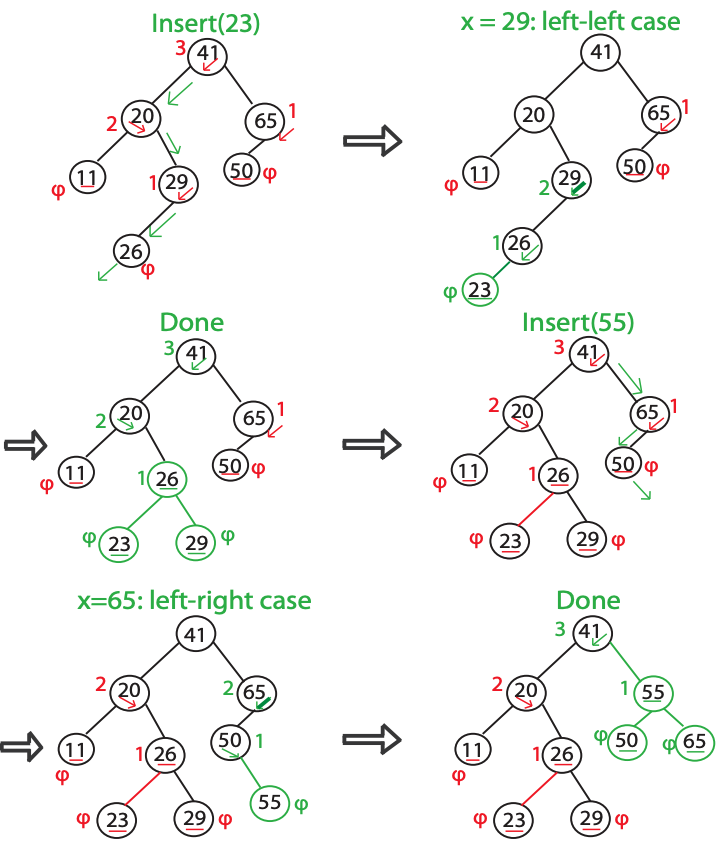
\includegraphics[width=0.65\textwidth]{exampleinsertbalancing.png}
    \end{minipage}
};

%------------ AVL Trees Header ---------------------
\node[fancytitle, right=10pt] at (box.north west) {AVL Tree Balancing};
\end{tikzpicture}

%------------ Red-Black Trees ---------------
\begin{tikzpicture}
\node [mybox] (box){%
    \begin{minipage}{0.3\textwidth}
    \textbf{Red-Black properties:}
    \footnotesize
    \begin{enumerate}
            \setlength{\itemsep}{-1mm} % Set the vertical space between items
            \item Every node is either red or black
            \item The root and leaves ($NIL$'s) are black.
            \item If a node is red, then its parent is black.
            \item All simple paths from any node $x$ to a descendant leaf have the same number of black nodes $=black-height(x)$.
        \end{enumerate}
        \textcolor{red}{\textbf{Theorem.}} A red-black tree with $n$ keys has height $$h \leq 2lg(n+1)$$
        \textcolor{blue}{\textbf{Proof.}} \footnotesize{Merge red nodes into their black parents $\rightarrow$ node has 2, 3 or 4 children. The 2-3-4 has uniform depth $h'$ of leaves.}
        $$n+1 \implies n+1\geq2^{h'} \implies lg(n+1)\geq h' \geq \frac{h}{2} $$
        $$ \implies h\leq 2 \ lg(n+1)$$

    
    \end{minipage}
};
%--------------RB Trees Header------------
\node[fancytitle, right=10pt] at (box.north west) {Red-Black Trees};
\end{tikzpicture}


%------------ RB Trees (cont'd) ---------------
\begin{tikzpicture}
\node [mybox] (box){%
    \begin{minipage}{0.3\textwidth}
        \footnotesize
        \textcolor{red}{Corollary.}The queries $SEARCH$, $MIN$, $MAX$, $SUCCESSOR$, and $PREDECESSOR$ all run in $O(lg \ n)$ time on a red-black tree with $n$ nodes
        \\
        0: Z= root ; 1: Z.uncle and parent = \textcolor{red}{red} \\ 2. Z.parent = \textcolor{red}{red}, uncle = black(triangle) ; 3. parent = \textcolor{red}{red}, Z.uncle = black(line)
        \begin{itemize}
            \setlength{\itemsep}{-1mm} % Set the vertical space between items
            \item 1: recolor Z's parent, grandparent, and uncle
            \item 2: rotate Z.parent
            \item 3: rotate Z.grandpa and recolor original parent and grandpa
        \end{itemize}


    \textbf{Analysis}
    \footnotesize
    \begin{itemize}
        \setlength{\itemsep}{-1mm} % Set the vertical space between items
        \item Go up the tree performing Case 1, which only recolors nodes
        \item If Case 2 or Case 3 occurs, perform 1 or 2 rotations, and terminate
    \end{itemize}
    \textcolor{red}{\textbf{Running time:}}$O(lg \ n)$ with $O(1)$ rotations.
    
    
    \end{minipage}
};
%------------ RB Trees Header ---------------------
\node[fancytitle, right=10pt] at (box.north west) {Red-Black Trees};
\end{tikzpicture}

%------------ Hash Tables ---------------
\begin{tikzpicture}
\node [mybox] (box){%
    \begin{minipage}{0.3\textwidth}
    \textcolor{red}{\textbf{\textit{Worst case:}}}
    \vspace{-10pt}
    \begin{itemize}
    \setlength{\itemsep}{-1mm} % Set the vertical space between items
        \item Every key hashes to the same slot.
        \item Access time $=O(n)$ if $|S| = n$
    \end{itemize}
    \textbf{Assume \textit{simple uniform hashing}}
    \\
    Let $n$ be the number of keys in the table, and $m$ be the number of slots.
    \\
    Define the \textit{load factor} of $T$ to be:
    $$\alpha = \frac{n}{m} = \text{average number of keys per slot} $$
    \\
    \textbf{Search Cost:} Expected time of \textit{unsuccessful} search for record with given key $= \Theta(1+\alpha)$
    
    \end{minipage}
};
%------------ Hash Tables Header ---------------------
\node[fancytitle, right=10pt] at (box.north west) {Hash Tables};
\end{tikzpicture}

%------------ Graphs - Intro ---------------
\begin{tikzpicture}
\node [mybox] (box){%
    \begin{minipage}{0.3\textwidth}
    \textbf{DFS} starting from node $v$ Running Time (without recursion): $\Theta(deg^+v)$
    \\
    \textbf{DFS} for all nodes of a graph. Running time: $\Theta(|V|+\sum_{v\in V}(deg^+(v)+1)) = \Theta(|V|+|E|)$
    \\
    \textbf{BFS} for all nodes of a graph. Running time: $\Theta(|V|+|E|)$
    \end{minipage}

};
%------------ Graphs-Intro Header ---------------------
\node[fancytitle, right=10pt] at (box.north west) {Graphs - Intro};
\end{tikzpicture}
%------------ Topsort ---------------------
\begin{tikzpicture}
\node [mybox] (box){%
    \begin{minipage}{0.3\textwidth}
        \begin{center}
            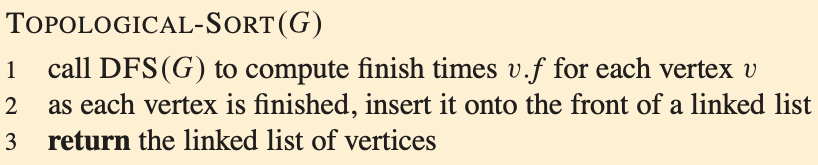
\includegraphics[width=1\textwidth]{topsort.png}
        \end{center}
        The procedure runs in $\Theta(V+E)$ time.\\
        \footnotesize($O(1)$ to insert nodes in linked list)
    \end{minipage}
};
%------------ Topsort ---------------------
\node[fancytitle, right=10pt] at (box.north west) {Graphs - Topological Sorting};
\end{tikzpicture}

%------------ BST Content ---------------
\begin{tikzpicture}
\node [mybox] (box){%
    \begin{minipage}{0.3\textwidth}
        \begin{minipage}{0.25\textwidth}
            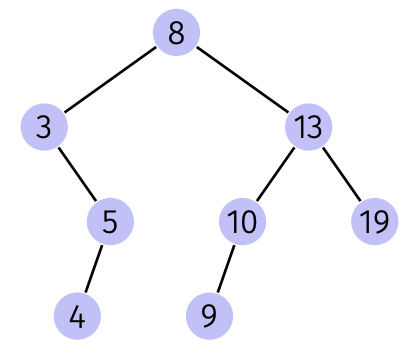
\includegraphics[width=1\textwidth]{bsttraversal.png}
        \end{minipage}
        \begin{minipage}{0.75\textwidth}
        \footnotesize
        \hspace{-20pt}
        \vspace{-0pt}
            \begin{itemize}
            \setlength{\itemsep}{-1mm} % Set the vertical space between items
                \item preorder: $v$, then $T_{left}(v)$, then $T_{right}(v)$.
                \subitem\textcolor{blue}{8, 3, 5, 4, 13, 10, 9, 19}
                \item postorder: $T_{left}(v)$, then $T_{right}(v)$, then $v$.
                \subitem\textcolor{blue}{4, 5, 3, 9, 10, 19, 13, 8}
                \item inorder: $T_{left}(v)$, then $v$, then $T_{right}(v)$.
                \subitem\textcolor{blue}{3, 4, 5, 8, 9, 10, 13, 19}
            \end{itemize}
        \end{minipage}
    \end{minipage}
};
%------------ BST Header ---------------------
\node[fancytitle, right=10pt] at (box.north west) {Binary Search Trees};
\end{tikzpicture}

%------------ SCC Content ---------------
\begin{tikzpicture}
\node [mybox] (box){%
    \begin{minipage}{0.3\textwidth}
    \footnotesize
    \begin{enumerate}
    \setlength{\itemsep}{-1mm} % Set the vertical space between items
        \item call DFS(G) from any vertex $v$ $O(V+E)$
        \item Insert each finished vertex in a stack $O(V)$
        \item "Calculate $G^R$ $O(E)$
        \item Apply DFS on $G^R$ following the stack in $2)$ $O(V+E)$
    \end{enumerate}
    \vspace{-5pt}
    The trees of the DFS in $4)$ are the SCC of $G$.
    \end{minipage}
};
%------------ SCC Header ---------------------
\node[fancytitle, right=10pt] at (box.north west) {Strongly Connected Components};
\end{tikzpicture}

%------------ Dijkstra's Content ---------------
\begin{tikzpicture}
\node [mybox] (box){%
    \begin{minipage}{0.3\textwidth}
        \begin{multicols*}{2}
            \begin{center}
                \includegraphics*[width=0.35\textwidth]{dijkstraQ.png}
                \includegraphics*[width=0.35\textwidth]{dijkstragraph.png}
            \end{center}

        \end{multicols*}
        $S: \{A, C, E, B, D\}$
        \\
        \includegraphics*[width=.7\textwidth]{analysisDijkstra.png}
        \begin{center}
            Time = $\Theta(V.T_{EXTR-MIN} + E.T_{DECR-KEY})$
        \end{center}
        \begin{center}
        \begin{tabular}{||c c c c||}
            \hline
            $Q$ & $T_{E-N}$ & $T_{D-K}$ & Total \\ [0.5ex]
            \hline\hline
            array & $O(V)$ & $O(1)$ & $O(V^2)$ \\
            binary heap & $O(lg V)$ & $O(lg V)$ & $O(Elg V)$ \\
            \hline
        \end{tabular}
        \end{center}

    \end{minipage}
};
%------------ Dijkstra's Header ---------------------
\node[fancytitle, right=10pt] at (box.north west) {Shortest Paths - Dijkstra};
\end{tikzpicture}


\
%------------ MST Content ---------------
\begin{tikzpicture}
\node [mybox] (box){%
    \begin{minipage}{0.3\textwidth}
        \footnotesize
        Prim's:
    \begin{enumerate}
        \item Start at a vertex, each time go to the unvisited vertex with the lowest edge weight
    \end{enumerate}
        Kruskal's:
    \begin{enumerate}
        \item Start at lowest weighted edge, and create one single tree with all the lowest weighted edges in order
    \end{enumerate}

    \end{minipage}
};
%------------ MST Header ---------------------
\node[fancytitle, right=10pt] at (box.north west) {MST - Prim's and Kruskal's Algo};
\end{tikzpicture}

\
%------------ Rolling Hash Content ---------------
\begin{tikzpicture}
\node [mybox] (box){%
    \begin{minipage}{0.3\textwidth}
    \footnotesize 
    In the Pattern Matching, input is text string T length n and pattern string P of length m $<$ n. Goal to determine if text has substring exactly equal to pattern.
    \\
    T:CMPLbSdG\textcolor{red}{CMPS}NEDQCMP
    \\
    P:CMPS
    \begin{algorithm}[H]
    \caption{PatternMatch1(T,P)}\label{alg:cap} \Comment{Tot: $O(mn)$}
    \begin{algorithmic}
    \For{$i=0$ to $n-m$} 
    \If {$T[i...i+m-1]==P$} \Comment{$O(m)$}
        \State\Return True
    \EndIf
    \EndFor \\
    \Return False
    
    \end{algorithmic}
    \end{algorithm}

    \vspace*{-12pt}
    \begin{algorithm}[H]
    \caption{PatternMatch2(T,P)}\label{alg:cap}
    \begin{algorithmic}
    \State $h_p$ = $hash(P)$ \Comment{$O(m)$}
    \For{$i=0$ to $n-m$} \Comment{$O(n)$}
    \State$h$ = $hash(T[i...i+m-1])$ \Comment{$O(m)$}
    \If {$h_p == h$} \Comment{$O(n)$}
        \State\Return True
    \EndIf
    \EndFor \\
    \Return False
    
    \end{algorithmic}
    \end{algorithm}

    \vspace*{-12pt}
    \begin{algorithm}[H]
    \caption{PatternMatch2(T,P)}\label{alg:cap} \Comment{Tot: $O(mn)$}
    \begin{algorithmic}
    \State $h_p$ = $hash(P)$ \Comment{$O(m)$}
    \For{$i=0$ to $n-m$} \Comment{$O(n)$}
    \State\If {$i=0$}
    \State$h$ = $hash(T[i...i+m-1])$ \Comment{$O(m)$ Once}
    \Else
    \State $h=h-h(T[i-1]) + h(T[1+m-1])$
    \EndIf
    \If {$h_p == h$} \Comment{$O(n)$}
        \State\Return True
    \EndIf
    \EndFor \\
    \Return False
    
    \end{algorithmic}
    \end{algorithm}

    \end{minipage}
};
%------------ Rolling Hash Header ---------------------
\node[fancytitle, right=10pt] at (box.north west) {Rolling Hash};
\end{tikzpicture}


\end{multicols*}
\end{document}
